\documentclass[twocolumn,astrosymb]{aastex631}

%% The default is a single spaced, 10 point font, single spaced article.
%% There are 5 other style options available via an optional argument. They
%% can be invoked like this:
%%
%% \documentclass[arguments]{aastex631}
%% 
%% where the layout options are:
%%
%%  twocolumn   : two text columns, 10 point font, single spaced article.
%%                This is the most compact and represent the final published
%%                derived PDF copy of the accepted manuscript from the publisher
%%  manuscript  : one text column, 12 point font, double spaced article.
%%  preprint    : one text column, 12 point font, single spaced article.  
%%  preprint2   : two text columns, 12 point font, single spaced article.
%%  modern      : a stylish, single text column, 12 point font, article with
%% 		  wider left and right margins. This uses the Daniel
%% 		  Foreman-Mackey and David Hogg design.
%%  RNAAS       : Supresses an abstract. Originally for RNAAS manuscripts 
%%                but now that abstracts are required this is obsolete for
%%                AAS Journals. Authors might need it for other reasons. DO NOT
%%                use \begin{abstract} and \end{abstract} with this style.
%%
%% Note that you can submit to the AAS Journals in any of these 6 styles.
%%
%% There are other optional arguments one can invoke to allow other stylistic
%% actions. The available options are:
%%
%%   astrosymb    : Loads Astrosymb font and define \astrocommands. 
%%   tighten      : Makes baselineskip slightly smaller, only works with 
%%                  the twocolumn substyle.
%%   times        : uses times font instead of the default
%%   linenumbers  : turn on lineno package.
%%   trackchanges : required to see the revision mark up and print its output
%%   longauthor   : Do not use the more compressed footnote style (default) for 
%%                  the author/collaboration/affiliations. Instead print all
%%                  affiliation information after each name. Creates a much 
%%                  longer author list but may be desirable for short 
%%                  author papers.
%% twocolappendix : make 2 column appendix.
%%   anonymous    : Do not show the authors, affiliations and acknowledgments 
%%                  for dual anonymous review.
%%
%% these can be used in any combination, e.g.
%%
%% \documentclass[twocolumn,linenumbers,trackchanges]{aastex631}
%%
%% AASTeX v6.* now includes \hyperref support. While we have built in specific
%% defaults into the classfile you can manually override them with the
%% \hypersetup command. For example,
%%
%% \hypersetup{linkcolor=red,citecolor=green,filecolor=cyan,urlcolor=magenta}
%%
%% will change the color of the internal links to red, the links to the
%% bibliography to green, the file links to cyan, and the external links to
%% magenta. Additional information on \hyperref options can be found here:
%% https://www.tug.org/applications/hyperref/manual.html#x1-40003
%%
%% Note that in v6.3 "bookmarks" has been changed to "true" in hyperref
%% to improve the accessibility of the compiled pdf file.
%%
%% If you want to create your own macros, you can do so
%% using \newcommand. Your macros should appear before
%% the \begin{document} command.
%%
\newcommand{\vdag}{(v)^\dagger}
\newcommand\aastex{AAS\TeX}
\newcommand\latex{La\TeX}

\newcommand{\code}[1]{\textbf{\texttt{#1}}}
\usepackage{CJKutf8}
\usepackage{bm}
\usepackage{appendix}

%% Reintroduced the \received and \accepted commands from AASTeX v5.2
\received{\today}
\revised{\today}
\accepted{\today}

\submitjournal{ApJ}

%% alias for citations
\defcitealias{Greco2018}{G18}

% \def\G18{\citetalias{Greco2018}}

\shorttitle{UDGs in MW analogs}
\shortauthors{Li et al.}
%%
%% You can add a light gray and diagonal water-mark to the first page 
%% with this command:
%% \watermark{text}
%% where "text", e.g. DRAFT, is the text to appear.  If the text is 
%% long you can control the water-mark size with:
%% \setwatermarkfontsize{dimension}
%% where dimension is any recognized LaTeX dimension, e.g. pt, in, etc.
%%
%%%%%%%%%%%%%%%%%%%%%%%%%%%%%%%%%%%%%%%%%%%%%%%%%%%%%%%%%%%%%%%%%%%%%%%%%%%%%%%%
\graphicspath{{./}{figures/}}
%% This is the end of the preamble.  Indicate the beginning of the
%% manuscript itself with \begin{document}.

\begin{document}
\begin{CJK*}{UTF8}{gbsn}

\title{Ultra Diffuse Galaxies associated with Milky-Way Analogs}

% \correspondingauthor{Jiaxuan Li}
\author[0000-0001-9592-4190]{Jiaxuan Li (李嘉轩)}
\affiliation{Department of Astrophysical Sciences, 4 Ivy Lane, Princeton University, Princeton, NJ 08544, USA}

\author[0000-0002-5612-3427]{Jenny E. Greene}
\affiliation{Department of Astrophysical Sciences, 4 Ivy Lane, Princeton University, Princeton, NJ 08544, USA}

\author[0000-0003-4970-2874]{Johnny Greco}
\affiliation{Department of Astrophysical Sciences, 4 Ivy Lane, Princeton University, Princeton, NJ 08544, USA}
\affiliation{Center for Cosmology and AstroParticle Physics (CCAPP), The Ohio State University, Columbus, OH 43210, USA}

\author[0000-0003-1385-7591]{Song Huang (黄崧)}
\affiliation{Department of Astrophysical Sciences, 4 Ivy Lane, Princeton University, Princeton, NJ 08544, USA}
\affiliation{Department of Astronomy and Tsinghua Center for Astrophysics, Tsinghua University, Beijing 100084, China}

\author{Peter Melchior}
\affiliation{Department of Astrophysical Sciences, 4 Ivy Lane, Princeton University, Princeton, NJ 08544, USA}
\author{Remy Joseph}
\affiliation{Department of Astrophysical Sciences, 4 Ivy Lane, Princeton University, Princeton, NJ 08544, USA}

%% I'd like to invite Shany?

%% Note that the \and command from previous versions of AASTeX is now
%% depreciated in this version as it is no longer necessary. AASTeX 
%% automatically takes care of all commas and "and"s between authors names.

%% AASTeX 6.31 has the new \collaboration and \nocollaboration commands to
%% provide the collaboration status of a group of authors. These commands 
%% can be used either before or after the list of corresponding authors. The
%% argument for \collaboration is the collaboration identifier. Authors are
%% encouraged to surround collaboration identifiers with ()s. The 
%% \nocollaboration command takes no argument and exists to indicate that
%% the nearby authors are not part of surrounding collaborations.

%% Mark off the abstract in the ``abstract'' environment. 
\begin{abstract}

\end{abstract}

\keywords{Low surface brightness galaxies (940), Dwarf galaxies (416), Galaxy properties (615), Galaxy abundances (574)}


\section{Introduction} \label{sec:intro}

In this work, we use the circularized effective radius $r_{\rm eff}$, defined as the $r_{\rm eff} = r_{\rm eff, sma} \sqrt{b/a}$, where $r_{\rm eff, sma}$ is the effective radius along the semi-major axis of the aligned elliptical isophotes, and $b/a$ is the axis ratio of the isophotes.

We adopt a $\Lambda$CDM cosmology from \citet{Planck15} with $\Omega_{\rm m}= 0.307$ and $H_0 = 67.7\ $km s$^{-1}$ Mpc$^{-1}$. We use the AB system \citep{Oke1983} for magnitudes. The stellar mass used in this work is based on a \citet{Chabrier2003} initial mass function.

\section{Data} \label{sec:data}
\subsection{Hyper Suprime-Camera data}
The Hyper Suprime-Camera Subaru Strategic Program Survey (\citealt{Aihara2018}; hereafter HSC survey)\footnote{\url{https://hsc-release.mtk.nao.ac.jp/doc/}} is an optical imaging survey using the 8.2-m Subaru telescope and the Hyper Suprime-Camera \citep{Miyazaki2012, Miyazaki2018}. The \texttt{Wide} layer is designed to cover $\sim 1000\ \rm{deg}^{2}$ of the sky in five broad bands ($grizy$), reaching a depth of $g=26.6$ mag, $r=26.2$ mag and $i=26.2$ mag ($5\sigma$ point source). HSC data are processed using \code{hscPipe}\footnote{\url{https://hsc.mtk.nao.ac.jp/pipedoc_e/}} \citep{Bosch2018}, which is a customized version of the Large Synoptic Survey Telescope (LSST) pipeline \citep{LSST-pipeline}\footnote{\url{https://pipelines.lsst.io/}}. 

In this work, we use the \code{Wide} layer data from Public Data Release 2 (PDR2, also known as \code{S18A}) of HSC \citealt{Aihara2018}. It covers $\sim 300\ \rm{deg}^2$ in all five bands, which is 1.5 times larger than the dataset analyzed in \citetalias{Greco2018}. One of the key improvements made in \code{S18A} is the sky background subtraction. Compared with previous data releases, \code{S18A} adopted a full focal plane sky subtraction algorithm to overcome the over-subtraction of local sky background around bright objects \citep{Aihara2018,Li2021}. The unprecedented depth and careful sky subtraction makes \code{S18A} an ideal dataset to search for low surface brightness galaxies. 

%HSC \code{S18A} also provides bitmasks indicating bad pixels, cosmic rays, edges of CCDs and pixels with source detection, helping us generate image masks when extracting surface brightness profiles (Section \ref{sec:hsc_methods}). In this paper, we use the \code{WIDE} layer data from \code{S18A} (\code{PDR2}). It covers $\sim 300$ deg$^2$ in all five bands. 

\subsection{NASA-Sloan Atlas}
We use the NASA-Sloan Atlas (NSA \footnote{\url{http://nsatlas.org}}, \citealt{Blanton2005,Blanton2011}) to select galaxies analogous to the Milky Way. NSA is a catalog of parameters of local galaxies derived from the Sloan Digital Sky Survey \citep[SDSS,][]{York2000}. We use the new version of NSA catalog (\code{v1\_0\_1}\footnote{\url{https://www.sdss.org/dr13/manga/manga-target-selection/nsa/}}) which contains about $640,000$ galaxies out to $z < 0.15$. It also includes elliptical Petrosian aperture photometry for galaxies, which is considered to be more reliable than the photometry used in older versions. In this paper, we use the stellar mass derived from the ellpitical Petrosian photometry using \code{kcorrect v4\_2}. The redshifts of galaxies in NSA come from several spectroscopic surveys, gas surveys, or direct distance measurements. 



\section{Methodology}

\subsection{Source Detection}\label{subsec:detection}

How does S18A search different from \citetalias{Greco2018}. 

\subsection{Matching with Milky-Way analogs}
The goal of this paper is to study the UDG population hosted by MW-like galaxies. However, the properties of MW itself vary in literature \citep{Licquia2015,Bland-Hawthorn2016}, and the definitions of MW analogs are also different among groups. In the SAGA survey \citep{SAGA-I,SAGA-II}, MW analogs are selected based on their absolute $K$-band magnitude $-23 > M_K > -24.6$, which is derived using abundance matching by assuming a simple galaxy-halo connection model (Fig 2 of \citealt{SAGA-I}). This luminosity range approximately corresponds to a stellar mass range of $10.2 < \log\, M_\star/M_\odot < 11.0$. They also require the MW analogs to be in isolation (without nearby bright galaxies) and lie in a redshift range of $0.005 < z < 0.01$ (20-40 Mpc). In the ELVES survey \citep{ELVES-I,ELVES-II,CarlstenELVES2022}, the requirements for MW-like host is loosened to be $M_K < -22.1$ ($M_\star > 10^{9.9}\ M_\odot$) because the probed volume by ELVES ($D<12$ Mpc) is smaller than that of SAGA. We choose the stellar mass range of MW analogs to be $10.2 < \log\, M_\star/M_\odot < 11.2$, which is simply a 1 dex bin centered at the measured stellar mass of the Milky Way ($\sim 10^{10.7}\ M_\odot$, \citealt{Licquia2015}). MW analogs selected using this definition is very close to those in SAGA but are slightly more massive than the ELVES hosts.

Since UDGs are relatively scarce in MW-like hosts \citep{SAGA-II,CarlstenELVES2022}, it is helpful to probe a larger volume to obtain good statistics. However, UDGs will be too small and faint to be detected in HSC images beyond certain distances. We choose our redshift range to be $0.01 < z < 0.04$, which makes sure that we can detect a significant number of faint dwarf galaxies around MW-like hosts. We exclude galaxies $z<0.01$ because 1) the number is very small; 2) their large angular size makes them shredded in deblending step, including them will introduce a lot of spurious LSB objects. Our MW analogs sample complements the ELVES sample and SAGA sample in redshift range. 

After applying the stellar mass and redshift cuts to the NSA catalog, there are 23,218 galaxies left. Then we match them to the LSBG catalog produced in Section \ref{subsec:detection} as follows. For a given MW-like host, we first calculate its virial radius $R_{\rm vir}$ assuming the stellar mass-halo mass relation in \citet{Behroozi2010}. It turns out that 40\% of hosts have virial radii larger than 300 kpc. Then we identify any LSBG that falls into the projected angular virial radius of the host. Then these LSBGs are associated with the host. We repeat this process for all hosts. If one LSBG is associated to multiple hosts, we assign it to the nearest host (normalized by the angular size of virial radius). In the end, we have 901 MW-like hosts and 8,367 LSBGs associated with them. 


\subsection{Modeling}


\begin{figure*}
	\vbox{ 
		%\vskip -10mm
		\centering
		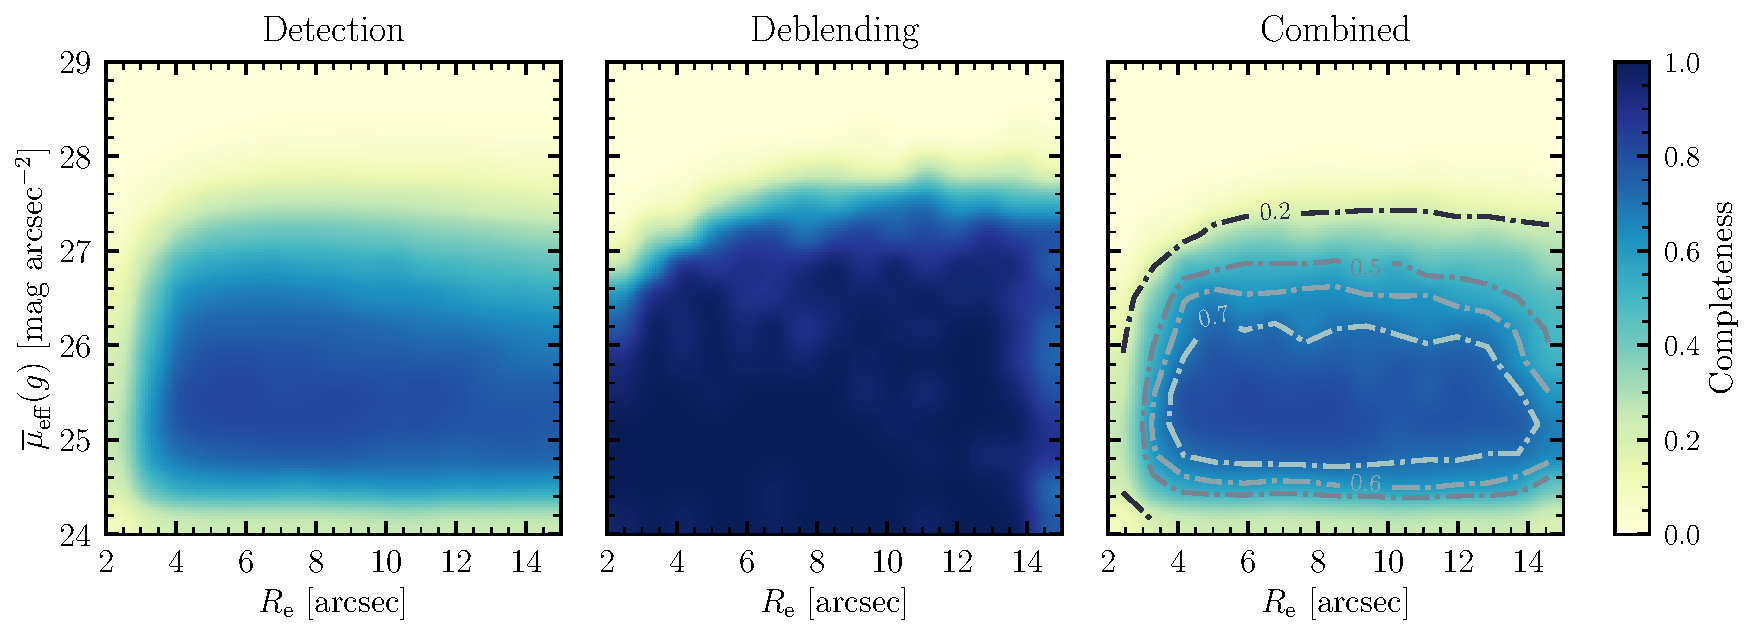
\includegraphics[width=1\linewidth]{completeness.pdf}
	}
	\caption{Caption}
	\label{fig:completeness}
\end{figure*}



\subsection{Measuring structural parameters}
Since the scarlet model is PSF-deconvolved, the color is not affected by the seeing differences among bands. 

\section{Ultra-diffuse galaxies in Milky-Way analogs}

\subsection{MW host selection}


\subsection{UDG sample}
Remember to filter the UDG sample through the FDFC mask, and also remove duplicated objects.
\begin{figure}
    \centering
    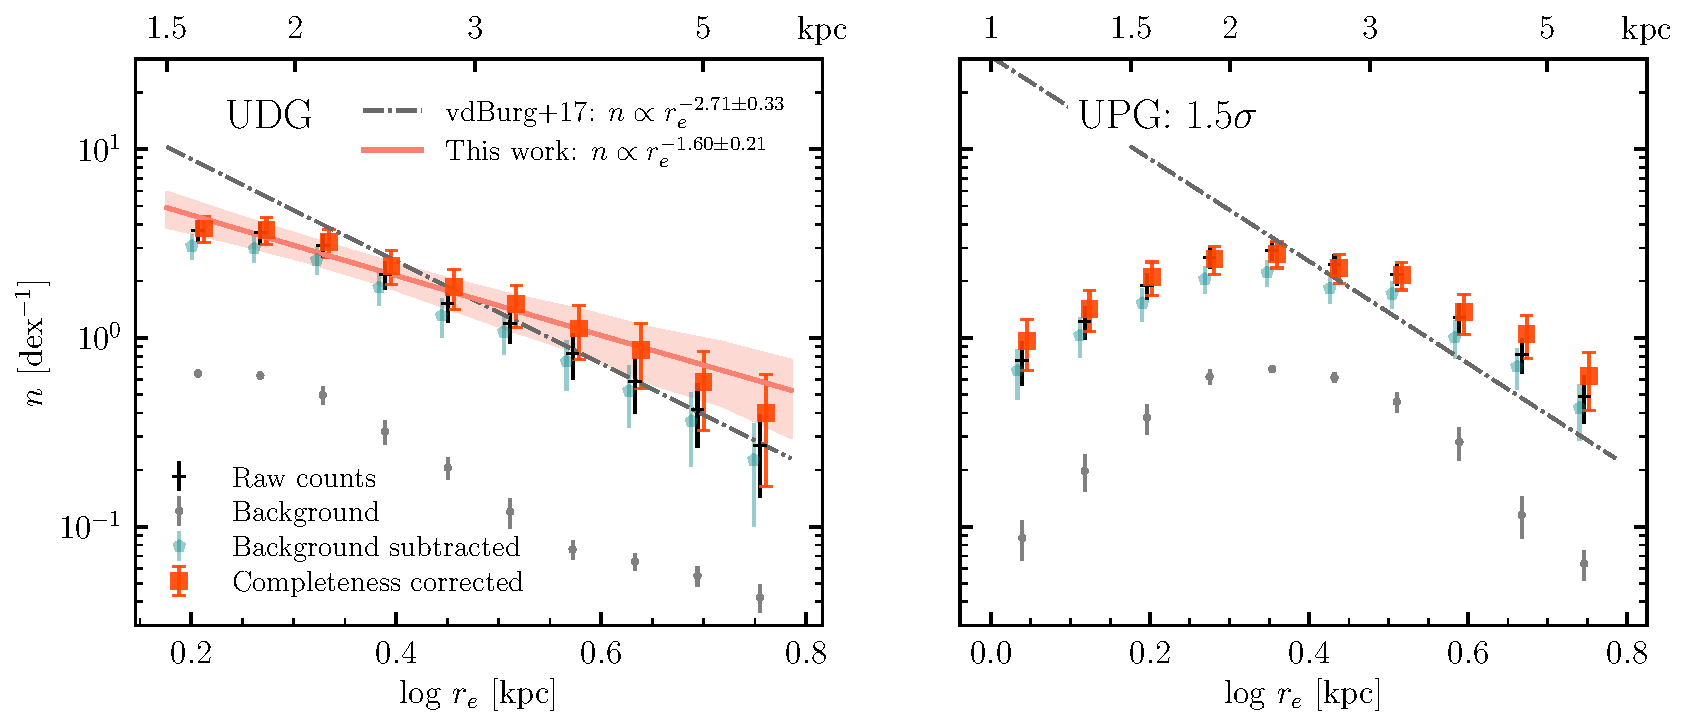
\includegraphics[width=1\linewidth]{size_distribution.pdf}
    \caption{Caption}
    \label{fig:size_distribution}
\end{figure}

\subsection{Spatial distribution}

\subsection{Quenched fraction}


\section{Discussion and Conclusion}
Scenarios:
1. violent environmental effects: radial orbits, back-splash both explain large size and quenching. But according to Bernavidis et al, the quenched fraction drops with increasing mass. 

2. accreting field UDGs, and quench them due to ram pressure stripping. But how long do accreted UDGs last before being destroyed? Need to look at ram pressure stripping literature.

Homework:
1. 1-sigma definition, UPG
2. number of UDG per host, as a function of host mass bins.
3. Move the stellar mass bin definition, try to match with red/blue, spiral/elliptical plot. If cannot match, does this hint the formation scenarios?
4. How significant do we detect blue UDGs? 
5. Split into redshift bins


UDG rejuvenate after ram pressure stripping?


Why red is equivalent to quenched? Need to clarify in the paper

calculate probability of being a backsplash satellite (e.g., splashed to 1.5 Mpc)

Compare spatial distribution with normal dwarf? iF they are indeed high-spin tail of normal dwarfs. 

\section*{Acknowledgment}
JL is grateful for discussions with XXX.

\software{\href{http://www.numpy.org}{\code{NumPy}} \citep{Numpy},
          \href{https://www.astropy.org/}{\code{Astropy}} \citep{astropy},  \href{https://www.scipy.org}{\code{SciPy}} \citep{scipy}, \href{https://matplotlib.org}{\code{Matplotlib}} \citep{matplotlib},
          \href{https://halotools.readthedocs.io/en/latest}{\code{Halotools}} \citep{Hearin2017}
          }


\bibliography{citation}{}
\bibliographystyle{aasjournal}



\newpage
\appendix 

\section{Mock galaxy tests}

vdB 16 doesn't consider whether GALFIT gives the corrrect $R_e$, when deriving the completeness (recovered fraction)

\subsection{Spergel profile}

\subsection{\code{scarlet} measurement error}

\begin{figure}
    \centering
    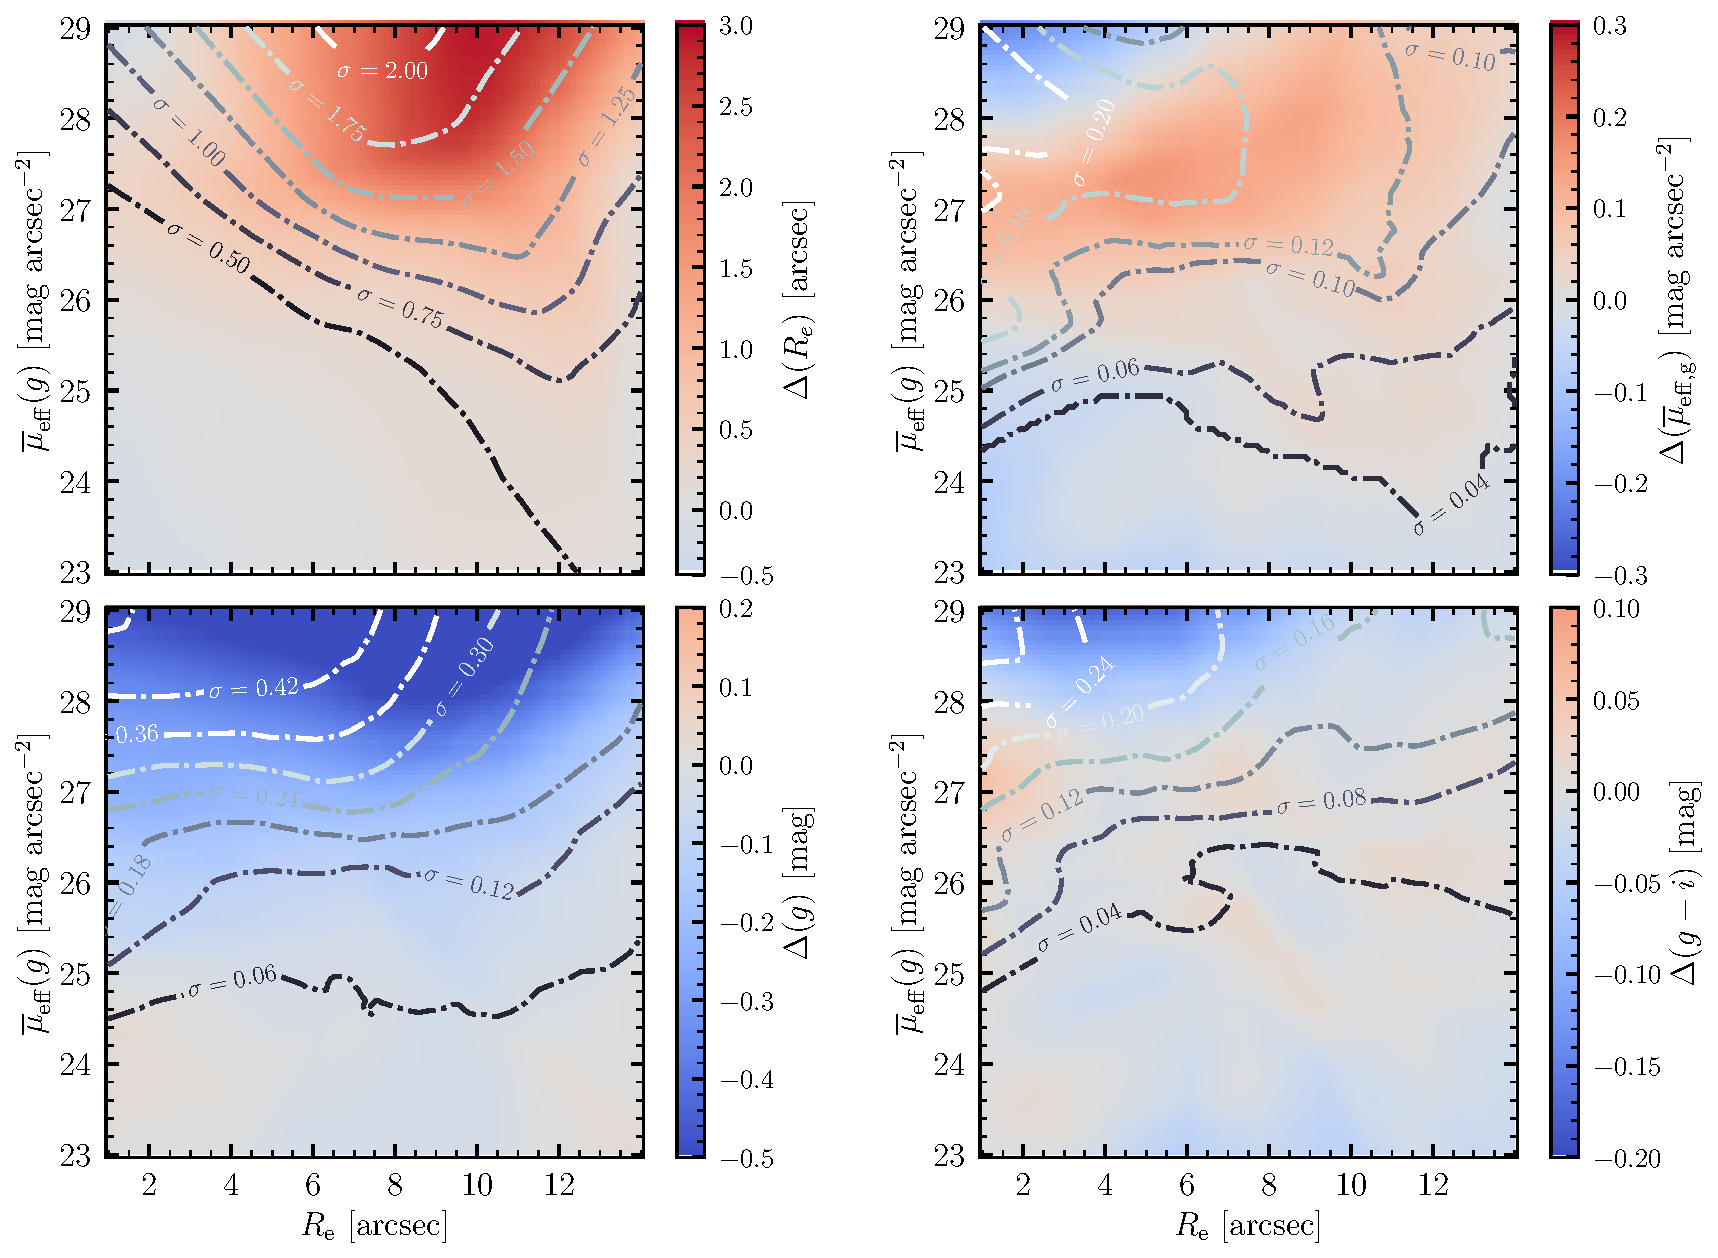
\includegraphics[width=1\linewidth]{meas_error_spergel.pdf}
    \caption{Caption}
    \label{fig:meas_err}
\end{figure}


%% This command is needed to show the entire author+affiliation list when
%% the collaboration and author truncation commands are used.  It has to
%% go at the end of the manuscript.
%\allauthors

%% Include this line if you are using the \added, \replaced, \deleted
%% commands to see a summary list of all changes at the end of the article.
%\listofchanges
\end{CJK*}
\end{document}

% End of file `sample631.tex'.
